\chapter{Komponenty}
\label{3-soucastky}

Při stavbě dronu je potřeba rozmyslet jeho účel, nosnost a délku letu. \cite{droncal}\\ Od těchto myšlenek (potřeb) se odvíjí dílčí součástky a jejich parametry. Základními součástkami jsou kostra, baterie, vrtule, motory, regulátory otáček, IMU, komunikační zařízení a řídící jednotka.\\
Důležitým faktorem je počet vrtulí/motorů. Podle počtu vrtulí dělíme drony na trikoptéry (3), quadrokopéry (4), hexakoptéry (6), a octokoptéry (8). Obecně platí, čím více má dron vrtulí, tím je stabilnější, dokáže létat i při selhání jednoho motorů (hexakoptéra a octokoptéra). Zároveň stavba dronu s vyšším počtem vrtulí je dražší a náročnější.\\
V této diplomové práci je popisována stavba hexakoptéry, jejíž kostra a motory byly použity z nefunkčního dronu of firmy Microkopter zapůjčeného z laboratoře fotogrammetrie.\\

\section{Kostra} 
Kostra by měla být lehká a pevná. Nejčastěji se používá karbon a hliník pro stavbu dronu s vyšší nosností a plast pro ostatní drony. Kostra se skládá z centra, ramen, stojánku a držáků pro motory.\\
Jak už bylo zmíněno, byla použita kostra od firmy Microkopter. Stojánek je vyroben z karbonu, centrum z plastu, ramena a držáky motorů z hliníku.\\


\section{Baterie} 
Výběrovým kritériem pro baterie jsou kapacita, výstupní napětí, maximální vybíjecí proud.
Nejpoužívanějšími bateriemi pro stavbu dronu jsou LiPo baterie, které nejsou těžké, nemají paměťový efekt, při správném zacházení mají dlouhou životnost a vysoký vybíjecí proud.\\
Výstupní napětí ovlivňuje množství článků baterie. Jeden článek má hodnotu nomi\-nálního napětí 3.7V, při plném nabití článku 4.2V. Maximální vybíjecí proud je dán konstantou C. Je-li konstanta C rovna 25 a kapacita baterie je 6750 mA, lze bezpečně odebírat proud o velikosti cca 168 Ampérů. Maximální odběr nesmí být větší, mohlo by dojít k poškození baterie.\\

\textbf{Výpočet proudového zatížení}
\begin{eqnarray*} 
	6.75A * 25C & = & 168.75A\\
\end{eqnarray*} 

\textbf{Parametry použité baterie}\\
%https://www.peckamodel.cz/ta-25c-6750-4s1p-gens-ace-lipo-tattu-serie-4s-6750-mah-25c\\
Počet článků: 4 (4S)\\
Napětí: 14.8V\\
Kapacita baterie: 6750mA\\
Maximální proudové zatížení: 25C (168.75A)\\
Maximální vybíjecí proud: 50C (337.5A)\\
Hmotnost: 605 g\\
Cena: 2500 Kč\\
\cite{baterie}\\

\textbf{Rady pro zacházení s LiPo bateriemi}\\
Nabíjet baterie proudem s 1C, tedy baterii s kapacitou 6750mA dobíjet proudem o velikosti 6.75A.\\
Nepřebíjet baterie nad hodnotu napětí 4.2V na článek.\\
Nepodbíjet baterie pod napětí 2.7V.\\
Při delším skladování vybít na hodnotu napětí 3.3V na článek.\\
Pro podrobnější instrukce je potřeba si přečíst příbalový leták.\\

\section{Distribuční deska} 
Distribuční deska PCB neboli napájecí deska slouží k zapojení všech  komponent na baterii. Jednotlivá napájená místa jsou zapojena paralelně, aby při zkratu jednoho ze zařízení, ostatní zařízení fungovala. K desce lze připojit i zařízení s jiným vstupním napětím než je napětí baterie (5V, 12V).\\

\textbf{Parametry distribuční desky}\\
Matek PDB-XT60\\
Množství LiPo článků: 3S-4S\\
Vstup VCC, GND\\
Výstup, 6x + a -, 12V, 5V, 2x -\\
Cena: 130 Kč\\
\cite{pdb}\\
%https://www.rotorama.cz/prislusenstvi/matek-pdb-s-5v-12v

\begin{figure}[H]
	\centering
	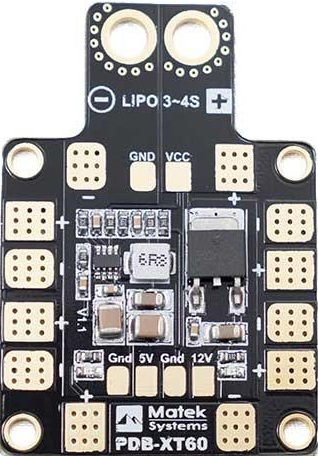
\includegraphics[width=3cm]{pictures/pdb.jpg}
	\caption{Distribuční deska - Matek PDB-XT60}
\end{figure}

\section{Vrtule} 
Vrtule generují tah dronu. Při stavbě dronu jsou potřeba dva typy vrtulí, se směrem hodinových ručiček a proti. Dva typy vrtulí jsou potřeba pro rotaci dronu kolem svislé osy. Další parametry jsou průměr a rozteč, nejčastěji uvedená v palcích. Materiál použivaný na výrobu vrtulí je plast nebo karbon. Doporučuji při stavbě dronu a jeho testování používat plastové vrtule, jsou cenově méně náročné.\\

\textbf{Parametry použitých vrtulí}\\
Materiál: plast\\
Průměr: 12 palců\\
Rozteč: 3.8 palce\\
Cena: 6 x 100 Kč\\

\section{Bezkartáčové motory} 
%https://www.youtube.com/watch?v=bCEiOnuODac
%learnengineering
%https://www.mikrocontroller.com/index.php?main_page=product_info&cPath=73&products_id=887&zenid=e5f2c8d548f2a39747a4ed06d306a37f
%motor
Motor se skládá z rotoru a statoru. Rotor je permanentní magnet, stator je prstenec uspořádaných cívek. Postupným pouštění proudu do cívek (vytvářením magnetic\-kého pole) se rotor začne pohybovat.\\
Cívky jsou rozdělené do skupiny A, B, C, což jsou i vstupní piny motorů.  Nedílnou součástí motorů je regulátor otáček ESC, který řídí vstupní proud přes piny A, B a C a tím ovlivňuje rychlost motoru. Prohozením pinů A a C určíme směr otáčení motoru, možnost otáčení lze změnit i při kalibraci regulátoru otáček.\cite{learnengineering}\\
Výběr motorů je závislý na konstatně Kv, parametrech baterie a parametrech re\-gulátoru otáček. Hodnota Kv neboli rpm/V je konstanta, která popisuje rychlost otáčení motoru v závislosti na napětí baterie. Platí úměra, čím menší je hodnota Kv, tím větší je tah motoru  a menší rychlost otáčení. Naopak čím  větší je hodnota Kv, tím je menší tah a větší rychlost otáčení. U závodních dronů se používají motory s větší hodnotou Kv, pro fotogrammetrii motory s menší hodnotou Kv.\cite{kv} \cite{siieefpv}\\

%http://learningrc.com/motor-kv/
%kn
%https://www.youtube.com/watch?v=y199oKTlwxU
%siieefpv
\textbf{Parametry použitých motorů}\\
Firma: Microkopter\\
Množství LiPo článků: 4S-6S\\
Provozní napětí: 25A\\
Maximální provozní napětí 30A\\
Rychlost bez zatížení: 500 rpm/V\\
Nosnost: 2200g\\
Váha: 121g\\
Cena: 6x 1500 Kč\\
\cite{motor}\\

\section{Regulátory otáček} 
Regulátory otáček (ESC) jsou nedílnou součástí BLDC motorů. Regulátor je řídící jednotka motoru, která zajistí plynulý chod. Regulátor se ovládá přes různé komunikační protokoly, které jsou popsány v kapitole Konstrukce.\\

\textbf{Parametry použitých regulátorů otáček}\\
HGLRC BS30A\\
Vnitřní software: BLHeliSuite\\
Vstup: VCC (7.4V - 18.5V) ,GND, -, S\\
Výstup: A, B, C\\
Maximální proud: 30A / 40A max\\
Množství LiPo článků: 2S-5S\\
Použitá knihovna: Servo\\
Cena: 200 Kč\\
\cite{esc}\\
%https://www.rotorama.cz/regulatory/hglrc-bs30a

\begin{figure}[H]
	\centering
	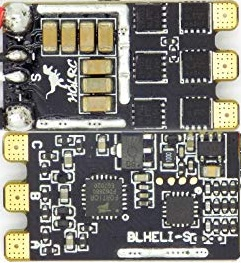
\includegraphics[width=4cm]{pictures/esc.jpg}
	\caption{Regulátor otáček - HGLRC BS30A}
\end{figure}

\begin{figure}[H]
	\centering
	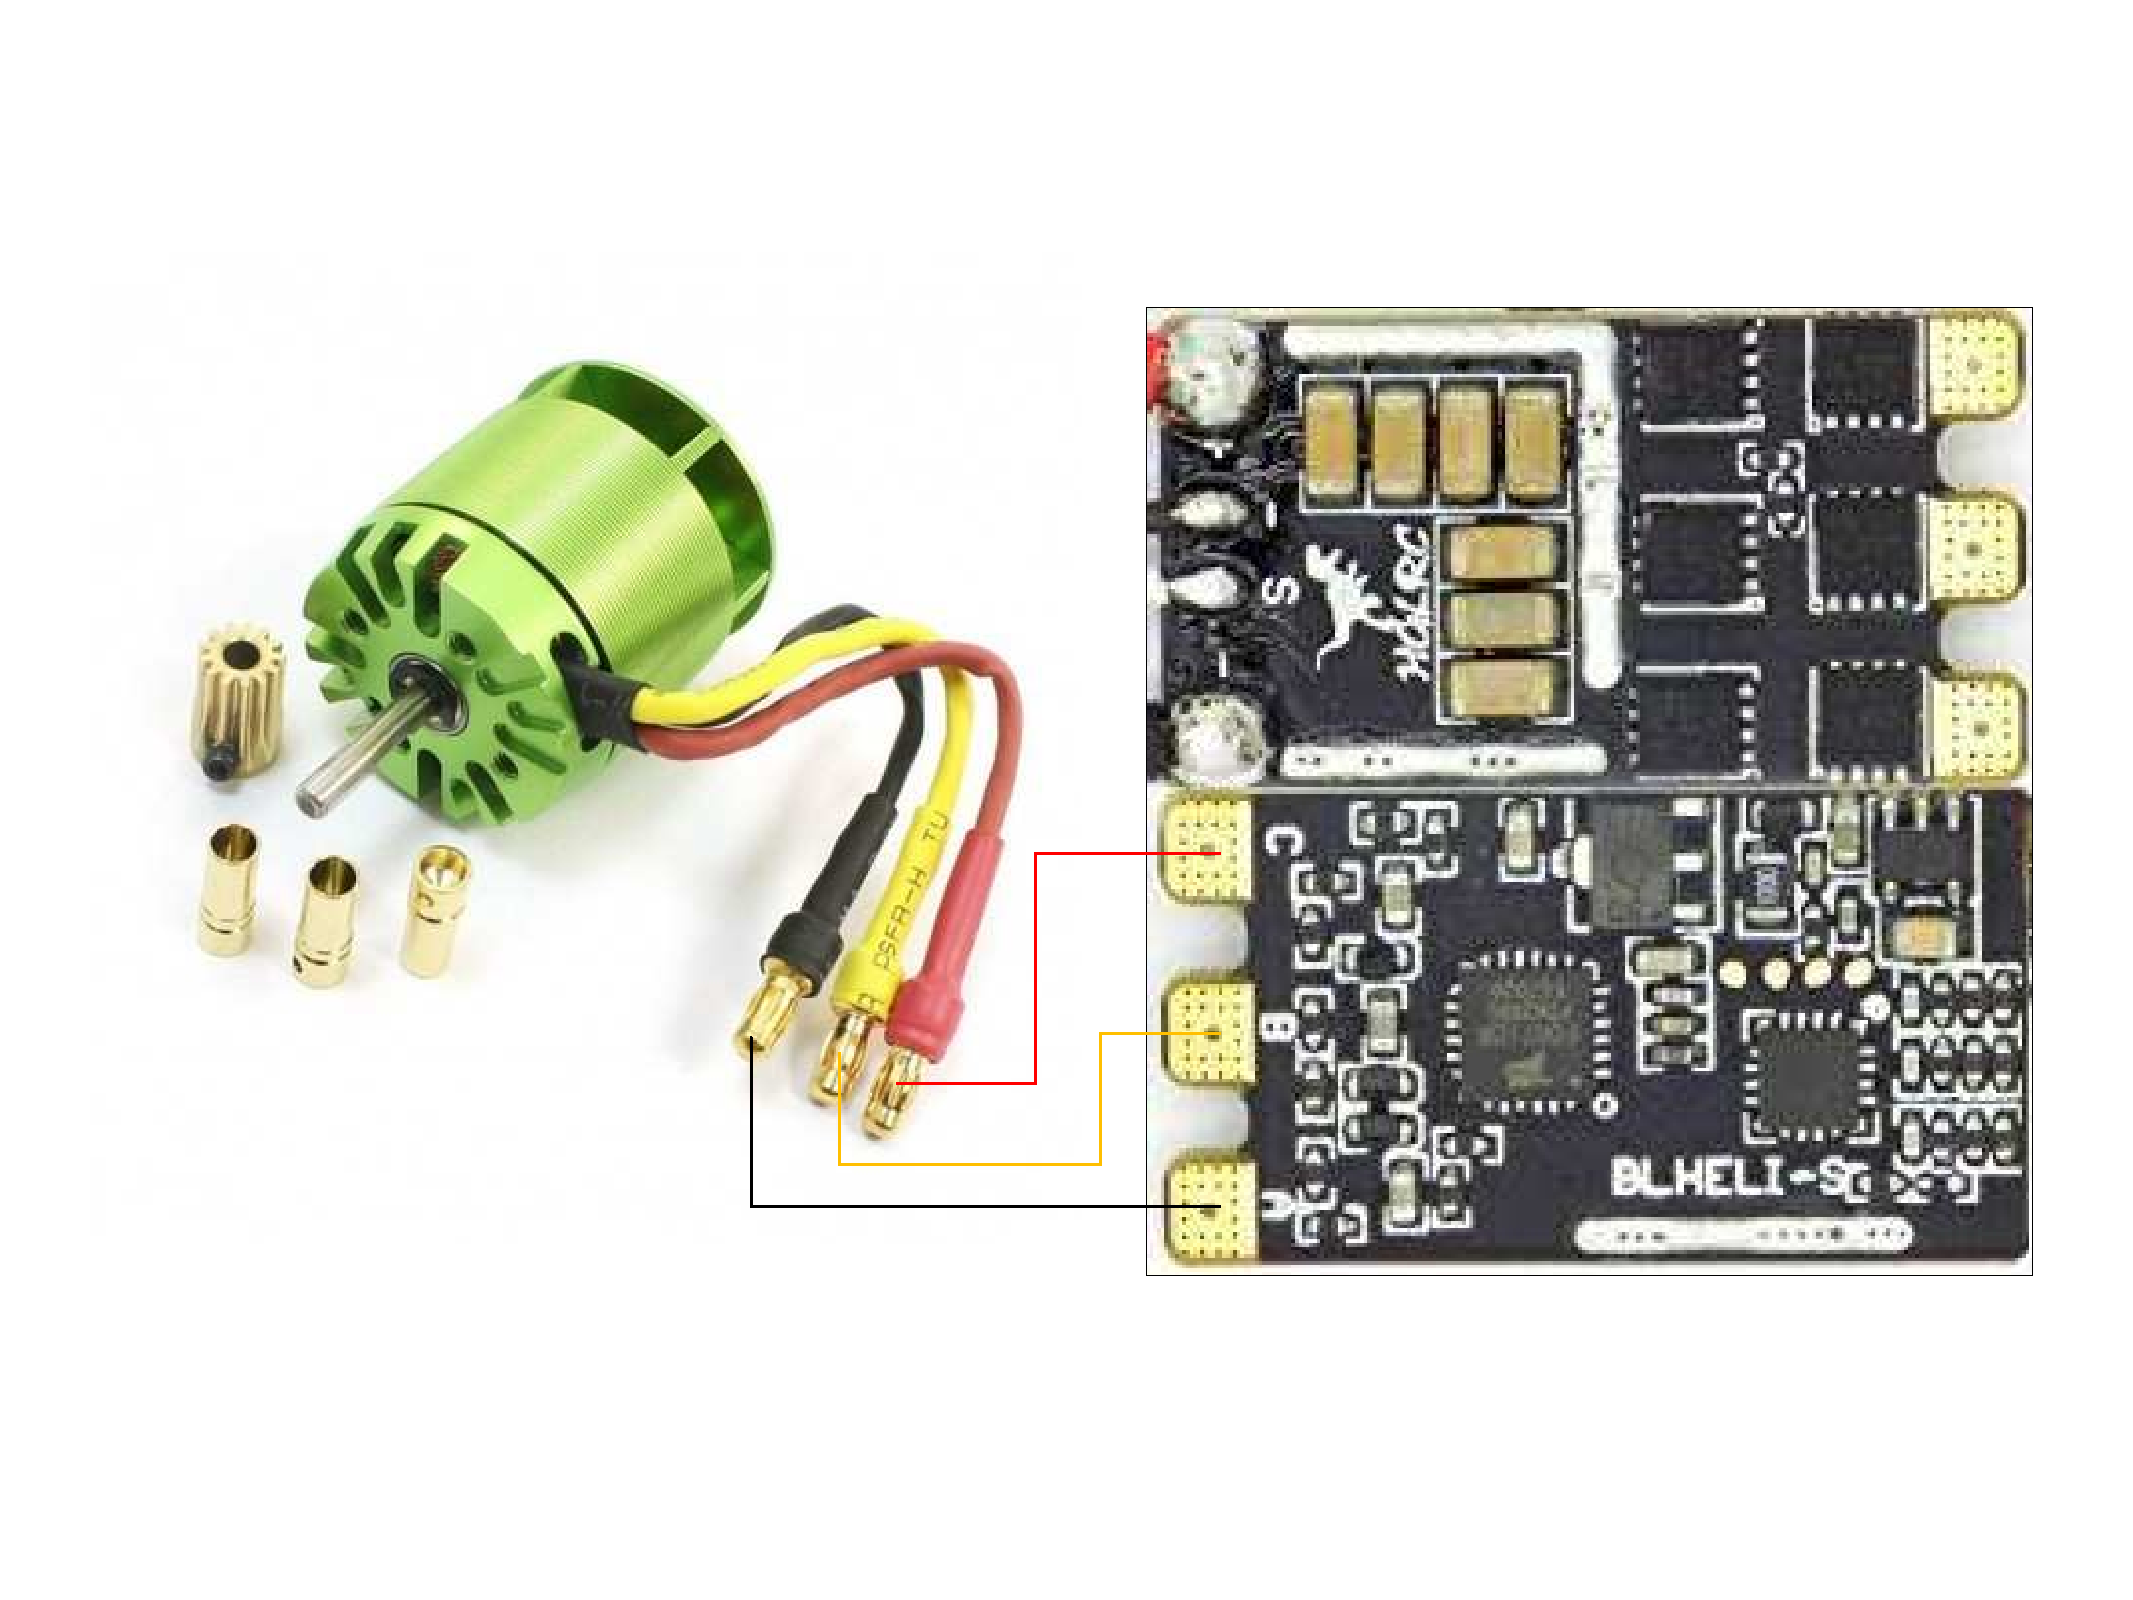
\includegraphics[width=8cm]{pictures/motor.pdf}
	\caption{Schéma zapojení motoru a regulátoru}
\end{figure}

\section{IMU}
IMU je zařízení, které měří úhlové rychlosti, zrychlení a orientaci v magnetickém poli ve třech osách. Skládá se z gyroskopu, akcelerometru a magnetometru. Všechna tři zařízení dohromady tvoří devět stupňů volnosti.  Použité IMU má shodný souřadný systém akcelerometru a gyroskopu, magnetometr má opačnou osu z a prohozené osy x a y.\cite{imu}\\

\subsection{Akcelerometr}
Akcelerometr slouží k určování zrychlení. Elektronický akcelerometr měří zrychlení na základě změny odporu mezi pevnou částí a pohyblivou částí akcelerometru. \\

\subsection{Gyroskop}
Gyroskop slouží k měření úhlové rychlosti.  Elektronický gyroskop měří úhlové rychlosti také na základě změny odporu, ale změnu měří ve dvou směrech na sobě kolmých. Z těchto dvou změn se vypočte úhel stočení.\\

\subsection{Magnetometr}
Magnetometr slouží k určování sil magnetického pole Země. Elektronický magnetometr využívá Hallův efekt, kdy vodivý plát je zasazen do elektronického obvodu. Při vlivu magnetického pole se na stranách plátu hromadí elektrony a protony. Měřené napětí na stranách plátu je úměrné k síle magnetického pole.\\

%https://www.youtube.com/watch?v=eqZgxR6eRjo&t=149s

\textbf{Parametry použité IMU jednotky}\\
Arduino modul MPU9250\\
Obsahuje: akcelerometr, gyroskop, magnetometr\\
Komunikace: I2C, SPI\\
Vstup: VCC (5V), GND\\
Výstup: SDA, SCL (I2C)\\
Cena: 300 Kč\\
\cite{mpu9250}\\
%https://www.invensense.com/wp-content/uploads/2015/02/PS-MPU-9250A-01-v1.1.pdf
%mpu9250
\begin{figure}[H]
	\centering
	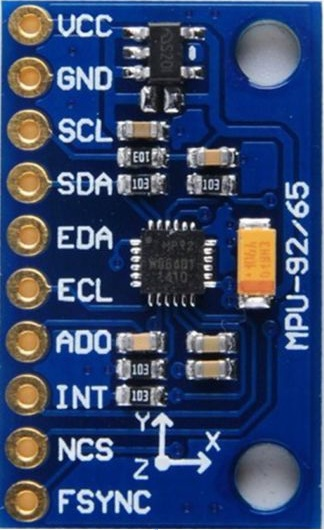
\includegraphics[width=3cm]{pictures/imu.jpg}
	\caption{IMU - MPU9250}
\end{figure}
 
\section{Komunikační zařízení} 
Pro bezdrátové ovládání dronu byl použit radiový modul a bluetooth.\\

\subsection{Radio} 
Radiový modul je používán pro zvětšení dosahu ovládání dronu. Pro stavbu byl použit bezdrátový modul XBee od firmy Digi. Modul plní funkce koncového zařízení, routeru nebo koordinátoru. Komunikace s XBee probíhá přes seriové rozhraní UART. Modul lze použít i pro čtení analogových a digitálních signálů různých senzorů.\\

\textbf{Parametry použitého Radiového zařízení}\\
XBEE PRO SS\\
Provozní napětí: 3.3V\\
Provozní frekvence: 2.4GHz\\
Komunikační protokol: ZB ZigBee\\
Dosah:1.5 km\\
\cite{xbee}\\

%https://www.proto-pic.co.uk/user/products/large/08665-03-L__99538__33841.jpg
\begin{figure}[H]
	\centering
	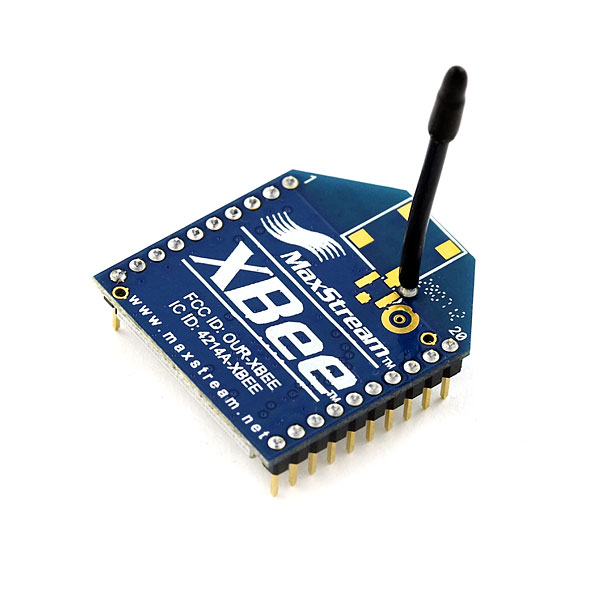
\includegraphics[width=5cm]{pictures/xbee.jpg}
	\caption{XBee}
\end{figure}

\subsection{Bluetooth} 
Pro bezdrátovou komunikaci s telefonem byl použit Arduino Bluetooth modul. Bluetooth modul využívá seriové rozhraní UART.\\

\textbf{Parametry použitého Bluetooth zařízení}\\
HC-05\\
Bluetooth verze: 2.0\\
Výchozí rychlost komunikace: 9600 baudů\\
Vstup: VCC (5V), GND, RX, EN\\
Výstup: TX, STATE\\
Použitá knihovna: SoftwareSerial\\
Cena: 200 Kč\\

\begin{figure}[H]
	\centering
	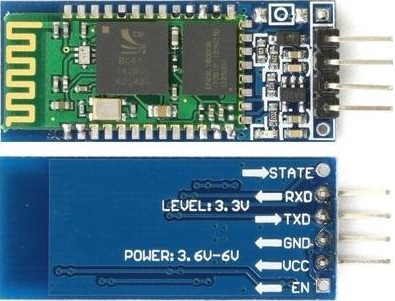
\includegraphics[width=5cm]{pictures/blue.jpg}
	\caption{Bluetooth - HC-05}
\end{figure}

\section{Řídící jednotka} 
Pro ovládání všech kompoment byla použita platforma Arduino.

\subsection{Arduino} 
Arduino je otevřená vývojová platforma, která využívá mikroprocesory od firmy \mbox{Atmel}. Programovat Arduino lze přes jazyk C nebo C++. Pro začínající uživatele byla vytvořena knihovna Wiring, která je velmi rozšířená. Knihovna je integrovaná do vývojového prostředí Arduino IDE. Na trhu existuje spousta typů desek např. Uno, Nano, Mega, Due. \\
Arduino lze napájet přes 12V konektor, USB nebo VIN, vstupní napětí je v rozsahu 5V - 12V. Vstupy Arduina jsou analogové, nebo digitální. Rozsah analogových \mbox{vstupů} je 0-1023. Digitální vstupy mají hodnotu LOW nebo HIGH, nominální napětí na pinech je 5V, pouze na Arduino DUE je hodnota napětí 3.3V. Desky podporují komunikaci přes PWM, I2C(piny SCL, SDA), SPI (piny SCLK, MOSI, MISO, SS) nebo UART (piny TX, RX). Pro každou komunikaci jsou definovány určité digitální piny.\\

\textbf{Použité desky Arduino}\\
Arduino Uno- (ATmega328, 8bit, 16 MHz, 700 Kč)\\
Arduino Nano- (ATmega328, 8bit, 16 MHz, 700 Kč)\\
Arduino Due- (AT91SAM3X8E, 32bit, 84 MHz, 900 Kč)\\
Cena: 200 - 1000 Kč\\

\begin{figure}[H]
	\centering
	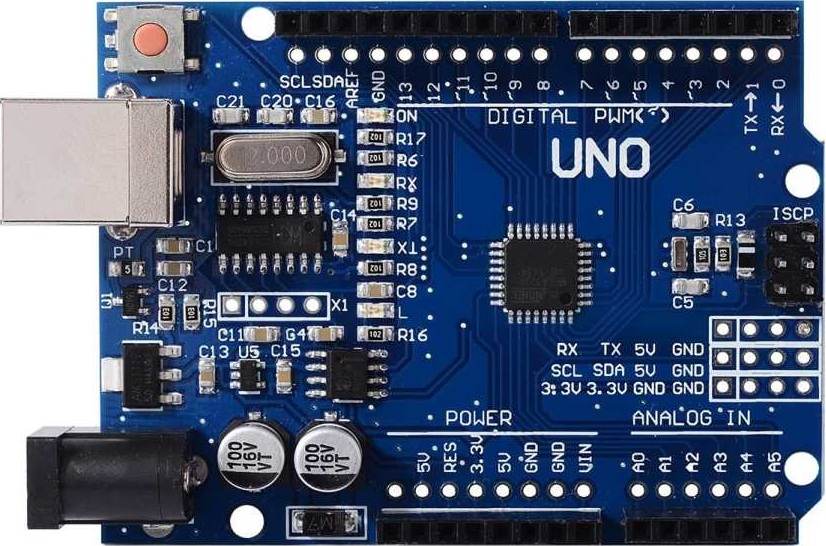
\includegraphics[width=5cm]{pictures/uno.jpg}
	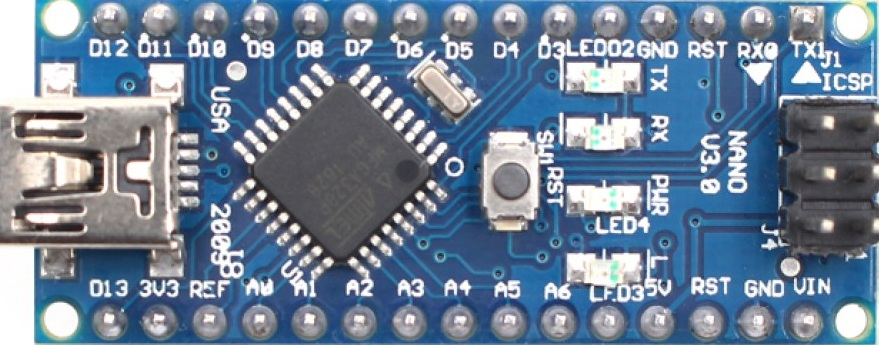
\includegraphics[width=5cm]{pictures/nano.jpg}
	\caption{Arduino UNO a Nano}
\end{figure}

\section{GNSS}
Při konstrukci měla být použita GNSS aparatura s podporou RTK z diplomové práce Štěpána Hodíka. Bohužel zatím není GNSS aparatura implementována.\\

\section{Výškoměr}
Pro funkci výškoměru byla požita dvě zařízení: barometr a GNSS.\\

\subsection{Barometr}
Barometrem měříme tlak. Z rozdílů tlaků na startovním místě a ve vzduchu lze spočítat výška letu dronu.\\

\textbf{Použitý barometr}\\
BMP280\\
Vstup: VCC (3.3V), GND,\\
Výstup: SDA, SCL, SDO, CSB\\
Měřící rozsah teploty:-40 až +85 stupňů\\
Měřící rozsah tlaku:300 až 1100 hPa\\
Přesnost měření teploty: +- 1 stupeň\\
Přesnost měření tlaku:  +- 100 Pa\\
Použitá knihovna: Adafruit BMP280\\
Cena: 80 Kč\\
\cite{bpm}\\
%https://github.com/adafruit/Adafruit_BMP280_Library

\begin{figure}[H]
	\centering
	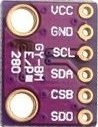
\includegraphics[width=2cm]{pictures/baro.jpg}
	\caption{Barometr - BMP280}
\end{figure}

\section{Laserový dálkoměr}
Pro automatizaci je důležité opatřit dron senzory měřící vzdálenosti pro detekci překážek. Senzory byly připevněny na ramena vrtulí pro měření vzdáleností ve vodorovné rovině a pro měření ve svislém směru pro přistávání a detekci objektů pod dronem. Použitý laserový dálkoměr měří vzdálenost pomocí tranzitního času.\\

\textbf{Použíty laserový modul}\\
laserový modul Vl53l0x\\
Vstup: VCC (5V), GND, XSHUT, GPIO1\\
Výstup: SDA, SCL (I2C)\\
vlnová délka: 940 nm\\
měřící rozsah: 0 - 1200 mm\\
přesnost: 3 procenta měřené délky\\
Použitá knihovna: VL53L0X\\
Cena: 230 Kč\\
\cite{laser}\\
%https://github.com/pololu/vl53l0x-arduino

\begin{figure}[H]
	\centering
	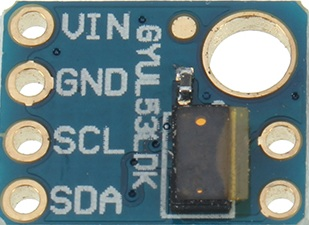
\includegraphics[width=2cm]{pictures/laser.jpg}
	\caption{Laserový modul - Vl53l0x}
\end{figure}

Při používání pouze jednoho modulu stačí propojit pouze 4 pin VIN, GND, SCL, SDA. Pro více modulů je potřeba zapojit pin XSHUT na některý z digitálních pinů. Všechny moduly mají továrně nastavenou totožnou adresu pro komunikaci. Pin XSHUT slouží k přepnutí modulu do stan-by režimu pro změnu adresy komunikace.\\ 

\section{Kamera}
Pro obrazový vjem letu dronu byl nainstalován systém FPV. FPV se skládá z kamery, vysílače, přijímače a obrazového media. Kamera předává obrazová data radiovému vysílači, který je na určité frekvenci posílá přijímači. Přijímač signál dekóduje a zobrazí na mediu.\\

\textbf{Použítá kamera}\\
Eachine TX02\\
Vstup: VCC (5V), GND\\
Výstup: radiový signál s frekvencí 5.8GHz\\
Zorné pole: 120 stupňů\\
Rozlišení: 600TVL\\
Použitá Android aplikace: FPViewer\\
Cena: 800 Kč\\

\begin{figure}[H]
	\centering
	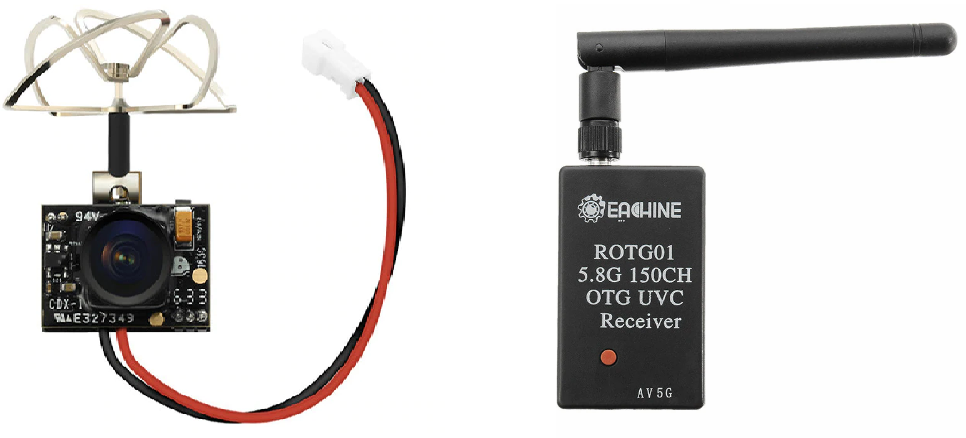
\includegraphics[width=10cm]{pictures/camera.png}
	\caption{Kamera TX02 s přijímačem pro smartphone}
\end{figure}